\section{Architecture}

%TODO Add project architecture (UML, SysUMl,...)

The rover itself consists of a python script that controls the hardware, provides a websocket for the camera feed and controls, and publishes sensor and actuator data to MQTT.
Another python script subscribes to this data from the rover and inserts it into a postgres database, which is then accessed by a Grafana dashboard (also running on the RPi).
Lastly, the browser accesses our web interface (which is running locally on the user's device for now), and establishes a websocket connection with the rover.

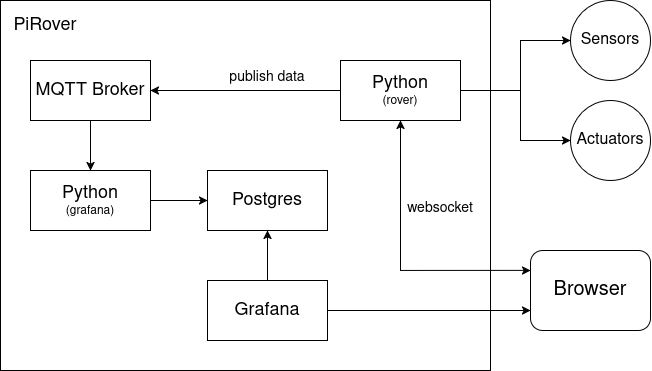
\includegraphics[width=0.8\textwidth]{img/architecture}
